Considere dois conjuntos quaisquer $X$ e $Y$ e um mapeamento $f$ do conjunto
$X$ para o conjunto $Y$. Se $f$ atribui um e apenas um valor para cada
elemento de $X$, dizemos que $f$ é uma função total e escrevemos $f: X \to Y$.
Chamamos $X$ de domínio de $f$, enquanto $Y$ é o contradomínio de $f$ e
$\forall x, (x \in X  \Rightarrow f(x) \in Y)$. Nesse sentido, $\forall x_1
\in X, \forall x_2 \in X, x_1 = x_2 \Rightarrow f(x_1) = f(x_2)$. Uma função
também pode ser parcial quando ela não é definida para alguns valores do
domínio. Escrevemos $f: X \nrightarrow Y $ para representar uma função parcial
definida em $A \subseteq X $, mas não definida no complementar de $A$. 

Um exemplo amplamente conhecido de funções parciais é $f: \mathbb{R}
\nrightarrow \mathbb{R}$, definida por $f(x) = \frac{1}{x}$, que é indefinida
em $x = 0$. Assim, na realidade, expressamos $f$ como $f : \mathbb{R}
\setminus \{0\} \to \mathbb{R}$. Alguns chamam $A$ de domínio de definição.
Como toda função parcial é total ao se restringir o domínio, trateremos nesse
texto das funções totais e a extensão das definições devido à parcialidade são
deixadas ao leitor.  

A maneira mais simples de se representar uma função é escrevê-la
explicitamente para cada elemento do domínio. Por exemplo, podemos escrever as
seguintes expressões:

\begin{itemize}
    \item Seja $f: \mathbb{N} \to \mathbb{N}$ definida por $f(n) = 2\cdot n +
    1$
    \item Seja $g : \mathbb{N} \to \mathbb{R}$ definida por $g(n) =
    \frac{n}{n+1}$
    \item Seja $h : \mathbb{R} \to \{0,1\}$ definida por
    $$\left \{ \begin{array}{c} h(x) = 1 ~if~x \in \mathbb{Q} \\
    h(x) = 0 ~ if ~ x \not \in \mathbb{Q} \\
    \end{array}
    \right. $$
 \end{itemize}

A questão que se levanta é: o que torna uma expressão explícita legítima?
Neste momento, deixaremos essa questão de lado e notaremos que a matemática é
confortável com diversos tipos de definições, como, por exemplo, a definição
de $h(x)$ no exemplo acima. Nesse mesmo exemplo, não fica claro em como
podemos definir algoritmicamente se um número real de entrada é um número
racional ou não. Porém, esse não é o objetivo do capítulo.

Note que a escolha das variáveis $x$ e $n$ são arbitrárias. Isto nos leva à
definição no Capítulo de \textit{\hyperlink{chapter.4}{FOL}} de variável
ligada (\textit{bound}), visto que se renomearmos $x$ com $y$, os valores
continuam os mesmos.

 Outra forma muito comum, principalmente na ciência da computação de definir
 funções é utilizando \textbf{recorrência}. Esse tipo de escrita é mais comum
 quando o domínio são os números naturais. Essas função são conhecidas como
 \textbf{sequências}. 

\begin{example}
     Considere $f: \mathbb{N} \to \mathbb{N}$, onde definimos $f(0) = 1$ e
     $f(n) = n\cdot f(n-1)$, para todo $n \in \mathbb{N}, n > 0$. Essa função
     é chamada de \textit{fatorial} de $n$. 
\end{example}

\begin{example}
    Considere $g: \mathbb{N} \to \mathbb{N}$, onde definimos $f(0) = 0$, $f(1)
   = 1$ e $f(n) = f(n-1) + f(n-2)$, para todo $n \in \mathbb{N}, n > 1$. Essa função
   é chamada de \textit{fibonacci}. Ela determina uma sequência conhecida, dada
   por $0, 1, 1, 2, 3, 5 ,8, ...$.  
\end{example}

Lógicos frequentemente utilizam a notação $\lambda x ~e(x)$ para denotar a
função que mapeia $x$ para $e(x)$. Essa notação chama-se \textit{notação
lambda} e pode ser usada da seguinte forma: $f = \lambda x(x + 1)$, que
significa $f(x) = x + 1$. Essa notação é mais interessante para cientistas da
computação e lógicos do que propriamente para matemáticos. Em Lean, definimos
da seguinte forma:

\begin{lstlisting}
variables X Y : Type
variable f : X → Y

def square (n : ℕ) := n*n 

def double (n : ℕ) := 2*n

variable n: ℕ 

#check square n     -- square n : ℕ 

#reduce square 3    -- 9

#eval square 12120  -- #reduce 12120 return an error, because the 
                    -- calculation is by deep recursion

example (n : ℕ) : double 2 = square 2 :=
by rw [double, square]
\end{lstlisting}

Lembre-se que diferenciamos o tipo $X$ do tipo $set~X$ em Lean.

Outra forma comum de representar funções de forma didática é utilizando
gráficos, como podemos observar na Figura \ref{fig:functions-01-00}. Essa
representação tem uma limitação muito clara que é quando $X$ é um conjunto
infinito. Um conjunto é finito quando existe um número natural $n$ tal que
exista uma função $b$ bijetiva entre esse conjunto e o conjunto dos números
naturais menores ou iguais a $n$. 

A definição de função bijetiva pode ser encontrada na Definiçao \ref{def7},
enquanto maiores informações sobre os números naturais podem ser encontradas
no Capítulo de \textit{\hyperlink{chapter.8}{Indução dos Números Naturais}}.
Conjuntos encontram-se no \textit{\hyperlink{chapter.5}{Capítulo 5}}.

A partir de agora, vamos introduzir uma série de definições sobre a
terminologia que de funções, que acabamos de apresentar, e vamos extrair
proposições importantes a partir. 

\begin{figure}
    \centering      
    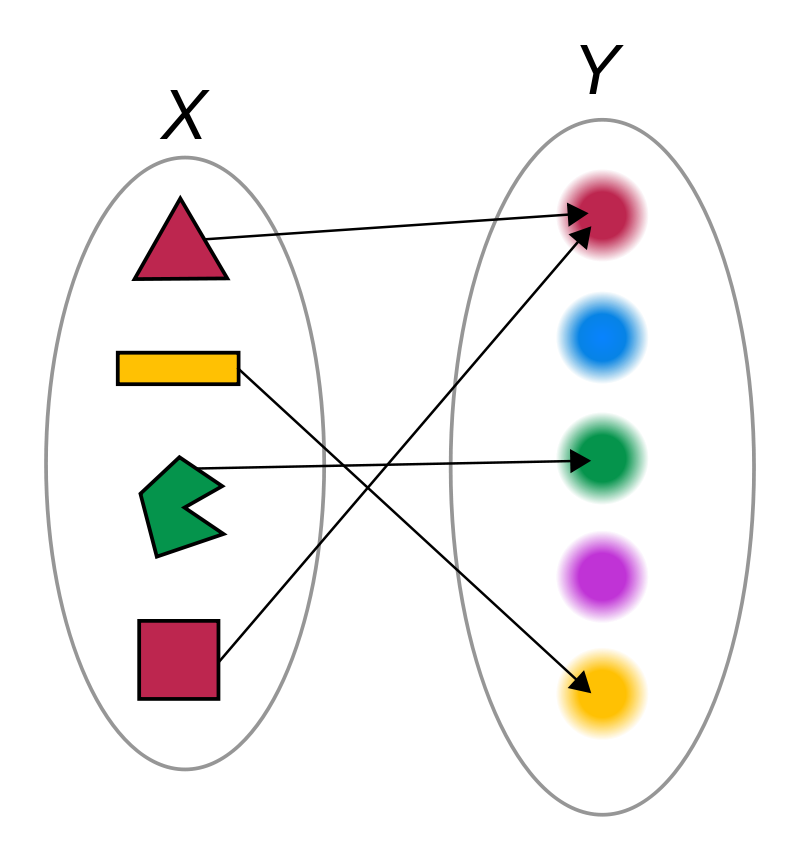
\includegraphics[width = 5cm]{figures/functions/fig-functions-01-00.png}
    \caption{Mapeamento entre o Domínio X e o Domínio Y, ambos não numéricos.}
    \label{fig:functions-01-00}
\end{figure}